\documentclass[fleqn, a4paper, 12pt, twoside]{article}
\usepackage{exsheets}
\usepackage{amsmath, amssymb, amsthm} %standard AMS packages
\usepackage{marginnote} %marginnotes
\usepackage{gensymb} %miscellaneous symbols
\usepackage{commath} %differential symbols
\usepackage{xcolor} %colours
\usepackage{cancel} %cancelling terms
\usepackage{siunitx} %formatting units
\usepackage{tikz, pgfplots} %diagrams
	\usetikzlibrary{calc, hobby, patterns, intersections}
\usepackage{graphicx} %inserting graphics
\usepackage{hyperref} %hyperlinks
\usepackage{datetime} %date and time
\usepackage{ulem} %underline for \emph{}
\usepackage{xfrac} %inline fractions
\usepackage{enumerate} %numbered lists
\usepackage{float} %inserting floats
\usepackage{circuitikz} %circuit diagrams
\usepackage{algpseudocode}
\usepackage{algorithm}

\newcommand\numberthis{\addtocounter{equation}{1}\tag{\theequation}} %adds numbers to specific equations in non-numbered list of equations

\newcommand{\AxisRotator}[1][rotate=0]{
	\tikz [x=0.25cm,y=0.60cm,line width=.2ex,-stealth,#1] \draw (0,0) arc (-150:150:1 and 1);%
} %rotation symbols on axes

\theoremstyle{definition}
\newtheorem{example}{Example}
\newtheorem{definition}{Definition}

\theoremstyle{theorem}
\newtheorem{theorem}{Theorem}

\newcommand{\curl}{\mathrm{curl\,}}

\newcommand{\Not}{{\textsc{not}}}
\renewcommand{\And}{{\textsc{and}}}
\newcommand{\Or}{{\textsc{or}}}
\newcommand{\Xor}{{\textsc{xor}}}

\newcommand{\AND}{\wedge}
\newcommand{\OR}{\vee}

\makeatletter
\@addtoreset{section}{part} %resets section numbers in new part
\makeatother

\newcommand\blfootnote[1]{%
	\begingroup
	\renewcommand\thefootnote{}\footnote{#1}%
	\addtocounter{footnote}{-1}%
	\endgroup
}

\SetupExSheets{solution/print = true}

%opening
\title{Digital Logic Systems}
\author{Aakash Jog}
\date{2014-15}

\begin{document}

\maketitle
%\setlength{\mathindent}{0pt}

\blfootnote
{	
	\begin{figure}[H]
		\includegraphics[height = 12pt]{cc.eps}
		\includegraphics[height = 12pt]{by.eps}
		\includegraphics[height = 12pt]{nc.eps}
		\includegraphics[height = 12pt]{sa.eps}
	\end{figure}
	This work is licensed under the Creative Commons Attribution-NonCommercial-ShareAlike 4.0 International License. To view a copy of this license, visit \url{http://creativecommons.org/licenses/by-nc-sa/4.0/}.
}

\tableofcontents

\newpage
\section{Lecturer Information}

\textbf{Prof. Guy Even}\\
~\\
Office: Wolfson 202\\
Telephone: 03-640-7769\\
E-mail: guy@eng.tau.ac.il\\

\section{Required Reading}

Guy Even and Moti Medina: \textit{Digital Logic Design}

\newpage
\part{Introduction to Discrete Math}

\section{Sets and Functions}

\begin{definition}[Universal set]
	The universal set is a set that contains all the possible objects.
\end{definition}

\begin{definition}[Set]
	A set is a collection of objects from a universal set.
\end{definition}

\begin{definition}[Subset]
	$A$ is a subset of $B$ if every element in $A$ is also an element in $B$. It is denoted as $A \subseteq B$
\end{definition}

\begin{definition}[Equal sets]
	Two sets $A$ and $B$ are said to be equal if $A \subseteq B$ and $B \subseteq A$.
\end{definition}

\begin{definition}[Strict containment]
	$A \subsetneq B \iff A \subseteq B \textnormal{ and } A \neq B$.
\end{definition}

\begin{definition}[Empty set]
	The empty set is the set that does not contain any element. It is usually denoted by $\emptyset$.
\end{definition}

\begin{definition}[Power set]
	The power set of a set $A$ is the set of all the subsets of $A$. The power set of $A$ is denoted by $P(A)$ or $2^A$.
\end{definition}

\begin{definition}[Ordered pair]
	Two objects (possibly equal) with an order (i.e., the first object and the second object) are called an ordered pair.
\end{definition}

\begin{definition}[Cartesian product]
	The Cartesian product of the sets $A$ and $B$ is the set 
	\begin{equation*}
		A \times B \triangleq \{ (a,b) | a \in A \textnormal{ and } b \in B \}
	\end{equation*}
\end{definition}

\begin{theorem}[De Morgan's Laws]\label{De Morgan's Laws}
	\begin{align*}
		\overline{A \cup B} &= \overline{A} \cap \overline{B}\\
		\overline{A \cap B} &= \overline{A} \cup \overline{B}
	\end{align*}
\end{theorem}

\begin{theorem}[Binary relation]
	A subset $R \subseteq A \times B$ is called a binary relation.
\end{theorem}

\begin{definition}[Function]
	A binary relation $R \subseteq A \times B$ is a function if for every $a \in A$ there exists a unique element $b \in B$ such that $(a,b) \in R$.
\end{definition}

\begin{definition}[Extension]
	Let $f$ and $g$ denote two functions. $g$ is an extension of $f$ if $f \subseteq g$, i.e., if every ordered pair in $f$ is also an ordered pair in $g$.
\end{definition}

\begin{definition}[Boolean function]
	A function B : {0, 1}n → {0, 1}k is called a Boolean function.
\end{definition}

\subsection{Important Boolean Functions}

\begin{definition}[$\Not$]
	\begin{equation*}
		\Not(x) = 1 - x
	\end{equation*}
\end{definition}

\begin{definition}[$\And$]
	\begin{equation*}
		\And(x) = x \cdot y
	\end{equation*}
\end{definition}

\begin{definition}[$\Or$]
	\begin{equation*}
		\Or(x) = x + y - (x \cdot y)
	\end{equation*}
\end{definition}

\begin{definition}[$\Xor$]
	\begin{equation*}
		\Xor(x) = (x + y) \bmod{2}
	\end{equation*}
\end{definition}

\section{Mathematical Induction}

\begin{theorem}
	For every $n \geq 2$, and for sets $A_1, \dots, A_n$,
	\begin{equation*}
		\overline{A_1 \cup \dots \cup A_n} = \overline{A_1} \cap \dots \cap \overline{A_n}
	\end{equation*}
\end{theorem}

\begin{proof}
	If $n = 2$, the statement is true, by \nameref{De Morgan's Laws}.\\
	Let
	\begin{equation*}
		B = A_1 \cup \dots \cup A_n
	\end{equation*}
	If possible, let
	\begin{align*}
		\overline{B} &= \overline{A_1} \cap \dots \cap \overline{A_n}
	\end{align*}
	Therefore,
	\begin{align*}
		\overline{A_1 \cup \dots \cup A_n \cup A_{n + 1}} &= \overline{B \cup A_{n + 1}}\\
		&= \overline{B} \cap \overline{A_{n + 1}}\\
		&= (\overline{A_1} \cap \dots \cap \overline{A_n}) \cap \overline{A_{n + 1}}
	\end{align*}
\end{proof}

\begin{theorem}[Pigeon-hole Principle]
	If there are $n$ holes and $m > n$ pigeons then there exists at least one hole with more than one pigeon in it. Let $f : A \to \{ 1,...,n \}$, and $|A| > n$, then $f$ is not one-to-one, i.e., there are distinct $a_1, a_2 \in A ; a_1 \neq a_2$, such that $f(a_1) = f(a_2)$.
\end{theorem}

\section{Sequences and Series}

\subsection{Sequences}

\subsubsection{Arithmetic Sequences}

\begin{definition}[Arithmetic Sequence]
	An arithmetic sequence $\left\{ a_n \right\}_{n = 0}^{\infty}$ is defined as
	\begin{equation*}
		a_n \doteq a_0 + n \cdot d
	\end{equation*}
\end{definition}

\subsubsection{Geometric Sequences}

\begin{definition}[Geometric Sequence]
	A geometric sequence $\left\{ b_n \right\}_{n = 0}^{\infty}$ is defined as
	\begin{equation*}
	b_n \doteq b_0 \cdot q^n
	\end{equation*}
\end{definition}

\subsection{Series}

\begin{definition}[Series]
	The sum of the elements of a sequence is called a series.
\end{definition}

\subsubsection{Arithmetic Series}

\begin{theorem}
	\begin{equation*}
		S_n = a_0 \cdot (n + 1) + d \cdot \dfrac{n (n + 1)}{2}
	\end{equation*}
\end{theorem}

\begin{proof}
	\begin{align*}
		S_n &= \sum_{i = 0}^{n} a_i\\
		&= \sum_{i = 0}^{n} a_n + i d\\
		&= \sum_{i = 0}^{n} a_0 + \sum_{i = 0}^{n} i d\\
		&= a_0 (n + 1) + d \sum_{i = 0}^{n} i\\
		&= a_0 (n + 1) + d \cdot \dfrac{n (n + 1)}{2}
	\end{align*}
\end{proof}

For estimation, 
\begin{align*}
	S_n &= \sum_{i = 0}^{n} a_i\\
	&\approx \int\limits_{0}^{n} f(x) \dif x\\
	&= \int\limits_{0}^{n} \left( a_0 + d \cdot x \right) \dif x\\
	\therefore S_n &\approx a_0 n + \dfrac{d}{2} n^2
\end{align*}

\subsubsection{Geometric Series}

\begin{theorem}
	\begin{equation*}
		S_n = b_0 \cdot \dfrac{q^{n + 1} - 1}{q - 1}
	\end{equation*}
\end{theorem}

For estimation,
\begin{align*}
	S_n &= \sum_{i = 0}^{n} b_i\\
	&\approx \int\limits_{0}^{n} g(x) \dif x\\
	&= \int\limits_{0}^{n} b_0 q^x \dif x\\
	\therefore S_n &\propto e^n
\end{align*}

\subsubsection{Harmonic Series}

\begin{theorem}
	Let
	\begin{equation*}
		H_n \doteq \sum_{i = 1}^{n} \dfrac{1}{i}
	\end{equation*}
	Then, $\forall k \in \mathbb{N}$,
	\begin{equation*}
		1 + \dfrac{k}{2} \leq H_{2^k} \leq k + 1
	\end{equation*}
\end{theorem}

\begin{proof}
	If $k = 0$,
	\begin{align*}
		H_{2^0} &= H_1\\
		&= 1\\
		\therefore 1 &\leq k + 1
	\end{align*}
	If possible, let $H_{2^k} \leq k + 1$.\\
	Therefore,
	\begin{align*}
		H_{2^{k + 1}} &= H_{2^k} + \sum_{i = 2^k + 1}^{2 \cdot 2^k} \dfrac{1}{i}\\
		\intertext{Therefore, by the induction hypothesis,}
		H_{2^{k + 1}} &\leq k + 1 + \sum_{i = 2^k + 1}^{2 \cdot 2^k} \dfrac{1}{i}\\
		\intertext{As the harmonic sequence monotonically decreases, the largest term between $2^k + 1$ and $2 \cdot 2^k$ is $\dfrac{1}{2^k}$. Therefore, $\sum\limits_{i = 2^k + 1}^{2 \cdot 2^k} \dfrac{1}{i} \leq \dfrac{1}{2^k} \cdot 2^k$. Therefore,}
		H_{2^{k + 1}} &\leq k + 1 + \dfrac{1}{2^k} \cdot 2^k\\
		\therefore H_{2^{k + 1}} &\leq k + 2
	\end{align*}
	Therefore, by induction,
	\begin{align*}
		H_{2^k} &\leq k + 1
	\end{align*}
	~\\
		If $k = 0$,
	\begin{align*}
		H_{2^0} &= 1\\
			&\geq 1 + \dfrac{k}{2}
	\end{align*}
	If possible, let $H_{2^k} \geq 1 + \dfrac{k}{2}$.\\
	Therefore,
	\begin{align*}
		H_{2^{k + 1}} &= H_{2^k} + \sum_{i = 2^k + 1}^{2 \cdot 2^k} \dfrac{1}{i}\\
		\therefore H_{2^{k + 1}} &\geq 1 + \dfrac{k}{2} + \dfrac{1}{2 \cdot 2^k} \cdot 2^k\\
		\therefore H_{2^{k + 1}} & \geq 1 + \dfrac{k}{2} + \dfrac{1}{2}\\
		\therefore H_{2^{k + 1}} & \geq 1 + \dfrac{k + 1}{2}
	\end{align*}
	Therefore, by induction,
	\begin{align*}
		H_{2^k} &\geq 1 + \dfrac{k + 1}{2}
	\end{align*}
	~\\
	Therefore,
	\begin{equation*}
		1 + \dfrac{k}{2} \leq H_{2^k} \leq k + 1
	\end{equation*}
\end{proof}

For estimation,
\begin{align*}
	H_n &\approx \int\limits_{1}^{n} \dfrac{1}{x} \dif x\\
	&= \ln x
\end{align*}

\section{Directed Graphs}

\begin{definition}[Directed graph]
	Let $V$ denote a finite set and $E \subset V \times V$. The pair $ G = (V,E)$ is called a directed graph. An element $v \in V$ is called a vertex or a node. An element $(u,v) \in E$ is called an arc or a directed edge.
\end{definition}

\begin{definition}[Path or walk]
	A path or a walk of length $l$ in a directed graph $G = (V,E)$ is a sequence $(v_0, e_0, v_1, e_1, \dots, v_{l - 1}, e_{l - 1}, v_l)$, such that
	\begin{enumerate}
		\item $v_i \in V \forall 0 \leq i \leq l$
		\item $e_i \in E \forall 0 \leq i < l$
		\item $e_i = (v_i, v_{i + 1}) \forall 0 \leq i < l$
	\end{enumerate}
\end{definition}

\begin{definition}[Closed path or cycle]
	A path is said to be closed if the first and last vertices are equal.
\end{definition}

\begin{definition}[Open path]
	A path is said to be open if the first and last vertices are distinct.
\end{definition}

\begin{definition}[Simple path]
	An open path is said to be simple if every vertex in the path appears only once in the path.
\end{definition}

\begin{definition}[Closed path]
	A closed path is said to be simple if every interior vertex appears only once in the path.
\end{definition}

\begin{definition}[Directed acyclic graph]
	A directed acyclic graph (DAG) is directed graph that does not contain any cycles.
\end{definition}

\begin{definition}[In-degree]
	The in-degree of a vertex $v$ is the number of edges that enter $v$. It is denoted as $\deg_{\textnormal{in}}(v)$.
\end{definition}

\begin{definition}[Out-degree]
	The out-degree of a vertex $v$ is the number of edges that enter $v$. It is denoted as $\deg_{\textnormal{out}}(v)$.
\end{definition}

\begin{definition}[Source and sink]
	A vertex is said to be a source if $\deg_{\textnormal{out}}(v) = 0$. A vertex is said to be a sink if $\deg_{\textnormal{in}}(v) = 0$.
\end{definition}

\begin{theorem}
	Each DAG has at least one sink.
\end{theorem}

\begin{theorem}
	Each DAG has at least one source.
\end{theorem}

\begin{definition}[Topological ordering]
	Let $G = (V,E)$ denote a DAG with $|V| = n$. A bijection $\pi : V \to \{0, \dots, n - 1\}$ is a topological ordering if $(u,v) \in E$ implies that $\pi(u) < \pi(v)$.
\end{definition}

\begin{algorithm}
	\caption{$\mathrm{TS}(V,E)$ - An algorithm for sorting the vertices of a DAG $G = (V,E)$ in topological ordering.}
	\begin{algorithmic}[1]
		\item Base Case: If $|V| = 1$, then let $v \in V$ and return $(\pi(v) = 0)$.
		\item Reduction Rule
			\begin{algorithmic}[1]
				\item Let $v \in V$ denote a sink and let $E_v$ denote any path which begins from or ends in $v$.
				\item return $(TS(V \setminus {v} , E \setminus E_v) \textnormal{ extended by } (\pi(v) =|V| - 1))$.
			\end{algorithmic}
	\end{algorithmic}
	\label{algorithm:TS(V,E)}
\end{algorithm}

\begin{theorem}
	$\mathrm{TS}(V,E)$ computes a topological ordering of a DAG $G = (V,E)$.
\end{theorem}

\begin{definition}[Longest path ending in a node]
	A path $\Gamma$ that ends in vertex $v$ is a longest path ending in $v$ if $|\Gamma'| \leq |\Gamma|$, for every path $\Gamma'$ that ends in $v$.
\end{definition}

\begin{definition}[Longest path]
	A path $\Gamma$ is a longest path if $|\Gamma'| \leq |\Gamma|$, for every path $\Gamma'$.
\end{definition}

\begin{theorem}
	If $G = (V,E)$ is a DAG, then there exists a longest path that ends in $v$, for every $v$. In addition, there exists a longest path in $G$.
\end{theorem}

\begin{algorithm}
	\caption{longest-path-lengths$(V,E)$ - An algorithm for computing the lengths of longest paths in a DAG. Returns a delay function $d(v)$.}
	\begin{algorithmic}[1]
		\item topological sort: $(v_0, \dots, v_{n−1}) \gets \textnormal{TS}(V, E)$.
		\item For j=0 to $(n−1)$ do
			\begin{algorithmic}[1]
				\item If $v_j$ is a source then $d(v_j) \gets 0$
				\item Else $d(v_j) \gets 1 + \max \{ d(v_i)∣i < j and (v_i,v_j) \in E \}$
			\end{algorithmic}
	\end{algorithmic}
\end{algorithm}

\section{Binary Representation}

\begin{definition}[Binary string]
	A binary string is a finite sequence of bits.
\end{definition}

\begin{definition}[Least significant and most significant bit]
	The least significant bit of the string $A[i : j]$ is the bit $A[k]$, where $k = \min \{i,j\}$. The most significant bit of the string A[i : j] is the bit A[l], where $l = \max \{i,j\}$.
\end{definition}

\begin{definition}[Binary number]
	The natural number $a$ is represented in binary representation by the binary string $A[n - 1 : 0]$ as
	\begin{equation*}
		a \doteq \sum_{i = 0}^{n - 1} A[i] \cdot 2^i
	\end{equation*}
	The term $2^i$ is called the weight of the bit $A[i]$.
\end{definition}

\begin{algorithm}
	\caption{$\mathrm{BR}(x,k)$ - An algorithm for computing a binary representation of a natural number $a$ using $k$ bits}
	\begin{algorithmic}[1]
		\If {$x \ge 2^k$}
			\State \Return fail
		\ElsIf {$k = 1$}
			\State \Return $x$
		\ElsIf {$x \ge 2^{k - 1}$}
			\State \Return $\left( 1 \circ \mathrm{BR} \left( x - 2^{k - 1}, k - 1 \right) \right)$
		\ElsIf {$x \le 2^{k - 1}$}
			\State \Return $\left( 0 \circ \mathrm{BR} \left( x, k - 1 \right) \right)$
		\EndIf
	\end{algorithmic}
\end{algorithm}

\section{Propositional Logic}

\begin{definition}[Constant or bit]
	A constant or a bit is either 0 or 1. As in the case of bits, 1 is interpreted as ``true” and a 0 as a “false”.The term bit is used in Boolean functions and in circuits while the term constants is used in Boolean formulas.
\end{definition}

\begin{definition}[Variable]
	A variable is an element in a set of variables. The set of variables is denoted by $U$. The set $U$ does not contain constants. Variables are usually denoted by upper case letters.
\end{definition}

\begin{definition}[Connectives]
	Connectives are operators used to build longer formulas from shorter ones. The set of connectives is denoted by $\mathcal{C}$.
\end{definition}

\begin{definition}[Arity]
	The arity of a connective is the number of operands or inputs that it accepts.
\end{definition}

\begin{definition}[Parse tree]
	A parse tree is a pair $(G, \pi)$ where $G = (V,E)$ is a rooted tree and $\pi : V \to \{0,1\} \cup U \cup \mathcal{C}$ is a labelling function that satisfies
	\begin{enumerate}
		\item A leaf is labelled by a constant or a variable, i.e. if $v \in V$ is a leaf, then $\pi(v) \in \{0,1\} \cup U$.
		\item An interior vertex $v$ is labelled by a connective whose arity is equal to the in-degree of $v$, i.e. if $v \in V$ is an interior vertex, then $\pi(v) \in \mathcal{C}$ is a connective with arity $\deg_{\textnormal{in}}(v)$.
	\end{enumerate}
\end{definition}

\end{document}